\ifx\boi\undefined\ifx\problemname\undefined
\providecommand\sampleinputname{}
\providecommand\sampleoutputname{}
\documentclass[lithuanian]{templates/boi}
\usepackage[L7x]{fontenc}
\problemlanguage{.lt}
\fi
\newcommand{\boi}{Baltijos šalių informatikos olimpiada}
\newcommand{\practicesession}{Bandomasis turas}
\newcommand{\contestdates}{2018 m. balandžio 27 - gegužės 1 d.}
\newcommand{\dayone}{1 diena}
\newcommand{\daytwo}{2 diena}
\newcommand{\licensingtext}{This problem is licensed under CC BY-SA 4.0.}
\newcommand{\problem}{Uždavinys}
\newcommand{\inputsection}{Pradiniai duomenys}
\newcommand{\outputsection}{Rezultatai}
\newcommand{\interactivity}{Realizacija}
\newcommand{\grading}{Vertinimas(?)}
\newcommand{\scoring}{Taškų skyrimas(?)}
\newcommand{\constraints}{Ribojimai}
\renewcommand{\sampleinputname}{Pradiniai duomenys}
\renewcommand{\sampleoutputname}{Rezultatai}
\newcommand{\sampleexplanation}[1]{Pirmojo pavyzdžio paaiškinimas}
\newcommand{\sampleexplanations}{Pavyzdžių paaiškinimai}
\newcommand{\timelimit}{Laiko ribojimas}
\newcommand{\memorylimit}{Atminties ribojimas}
\newcommand{\seconds}{s}
\newcommand{\megabytes}{MB}
\newcommand{\group}{Grupė}
\newcommand{\points}{Taškai}
\newcommand{\limitsname}{Ribojimai}
\newcommand{\additionalconstraints}{Papildomi ribojimai}
\newcommand{\testgroups}{
Jūsų sprendimas bus testuojamas su keliomis testų grupėmis, kiekviena kurių vertinama tam tikru skaičiumi taškų.
Kiekvieną testų grupę sudarys keletas testų.
Taškai už testų grupę skiriami tik jei įveikiate visus tos grupės testus.
}
\fi
\def\version{jury-1}
\problemname{Kintamoji srovė}
Fredrikas namuose žaidžia savo suprojektuotu geležinkelio modeliu, kuriuo jis labai didžiuojasi.
Geležinkelį sudaro $N$ segmentų, sujungtų į apskritimą, ir sunumeruotų $1, 2, \dots, N$ pagal laikrodžio rodyklę.
Elektra traukiniui tiekiama $M$ kabelių, nutiestų virš apskritimo, kuriuo eina geležinkelio bėgiai. 
Kiekvienam segmentui yra bent vienas kabelis, nutiestas virš to segmento.

Fredrikui pabodo ratu važinėjantis traukinys ir jis nutarė prie kiekvieno segmento pridėti po \emph{jungiklį}, kuriais naudodamasis jis galėtų nuversti traukinį nuo bėgių ar sukelti kitus įdomius įvykius. Tačiau jungikliams irgi reikia tiekti elektrą.
Ir ne bet kokią, o \emph{kintamos srovės}.\footnote{Tai logiška, nes šis geležinkelio modelis yra švediškas, o Švedijoje visi traukinių jungikliai (``växlar'') naudoja kintamą srovę (``växelström'').}


Fredrikas gaus kintamą srovę, jei turės abiem kryptimis tekančią srovę. Kiekvienu kabeliu srovė teka tik viena kryptimi (prieš ar pagal laikrodžio rodyklę), tačiau Fredrikas gali parinkti kryptį, kuria tekės srovė. Taigi, jis nori parinkti srovės tekėjimo kryptį kiekviename kabelyje taip, kad kiekvienas bėgių segmentas būtų uždengtas ir pagal, ir prieš laikrodžio rodyklę einančią srovę duodančiais kabeliais.

Padėkite Fredrikui išspręsti šį uždavinį.

\vspace{2mm}
%\hspace*{2mm}
\begin{center}
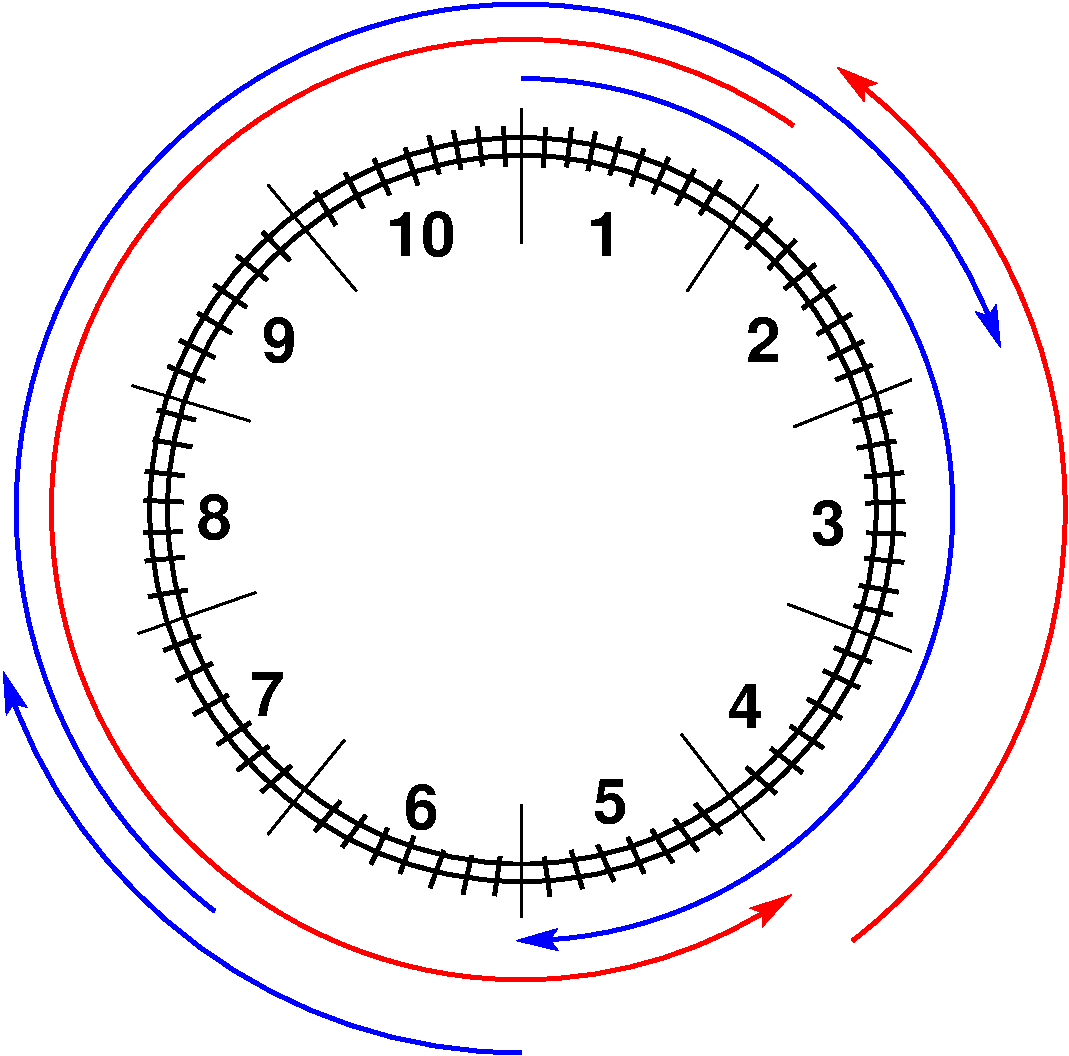
\includegraphics[width=0.5\textwidth]{alternatingfig.pdf}
\end{center}
\vspace{1mm} 
{\em Pirmojo pavyzdžio sprendimas. Išlenktos rodyklės reiškia elektrą tiekiančius kabelius. 
Rodyklės kryptis nurodo Fredriko pasirinktą elektros srovės kryptį (mėlyna ir raudona spalvos paryškina priešingas kryptis). Atkreipkite dėmesį, kad apsukę visas rodykles, gautume kitą galimą sprendimą: \texttt{11010}.}

\section*{\inputsection}
Pirmoje eilutėje pateikti du sveikieji skaičiai $N$ ir $M$ -- segmentų ir kabelių skaičius.

Kiekvienoje tolesnių $M$ eilučių yra po du skaičius $1 \le a, b \le N$, nurodančius, kad yra kabelis, dengiantis segmentus $a, a+1, \dots, b$. Jei $b$ mažesnis nei $a$, tai reiškia, kad dengiami segmentai $a, \dots, N, 1, \dots, b$. Tačiau jei $a=b$, kabelis dengia tik vieną segmentą.

\section*{\outputsection}
Išveskite vieną eilutę su $M$ simbolių, kurie būtų \texttt{0} arba \texttt{1}. $i$-asis eilutės simbolis turi būti \texttt{0}, jei $i$-uoju kabeliu srovė teka pagal laikrodžio rodyklę, arba \texttt{1}, jei ji teka prieš laikrodžio rodyklę.
Jei yra daugiau nei vienas galimas sprendinys, išveskite bet kurį.

Jei sprendinys neegzistuoja, išveskite ``\texttt{impossible}''.

\section*{\constraints}
\testgroups

\noindent
\begin{tabular}{| l | l | l | l |}
\hline
\textbf{\group} & \textbf{\points} & \textbf{\limitsname} & \textbf{\additionalconstraints} \\ \hline
  1     & 13     & $2 \le N, M \le 15$ & \\ \hline
  2     & 20     & $2 \le N, M \le 100$ & \\ \hline
  3     & 22     & $2 \le N, M \le 1000$ & \\ \hline
  4     & 19     & $2 \le N, M \le 100\,000$ & Jokiam kabeliui negalioja $b < a$. \\ \hline
  5     & 26     & $2 \le N, M \le 100\,000$ & \\ \hline
\end{tabular}

